\documentclass[11pt, a4paper]{article}

% ============================================
% PACKAGES
% ============================================
\usepackage[utf8]{inputenc}
\usepackage[T1]{fontenc}
\usepackage{mathptmx} % Times font
\usepackage[top=0.6in, bottom=0.6in, left=0.75in, right=0.75in]{geometry}
\usepackage{titlesec}
\usepackage{xcolor}
\usepackage{hyperref}
\usepackage{enumitem}
\usepackage{graphicx}
\graphicspath{{figures/}}
\usepackage{fancyhdr}
\usepackage{lastpage}
\usepackage{parskip}
\setlength{\parskip}{0.35em}
\setlength{\parindent}{0pt}
\usepackage{microtype}
\usepackage{wrapfig}
\usepackage{tikz}
\usepackage{caption}
\captionsetup{font=small, labelfont=bf, skip=4pt}

% ============================================
% COLOR DEFINITIONS (Johns Hopkins Blue Theme - matching Cover Letter)
% ============================================
\definecolor{accentcolor}{RGB}{0, 45, 114}     % JHU Dark Blue
\definecolor{darkaccent}{RGB}{0, 35, 90}       % Darker blue
\definecolor{lightaccent}{RGB}{200, 216, 235}  % Light blue background
\definecolor{linkcolor}{RGB}{0, 114, 178}      % Links (brighter blue)
\definecolor{textgray}{RGB}{60, 60, 60}        % Body text

% ============================================
% HYPERREF SETUP
% ============================================
\hypersetup{
    colorlinks=true,
    linkcolor=linkcolor,
    urlcolor=linkcolor,
    citecolor=linkcolor,
    pdftitle={Research Statement - Jie Gao},
    pdfauthor={Jie Gao}
}

% ============================================
% HEADER AND FOOTER
% ============================================
\pagestyle{fancy}
\fancyhf{}
\renewcommand{\headrulewidth}{0pt}
\fancyhead[L]{\small\color{textgray}Jie Gao}
\fancyhead[R]{\small\color{textgray}Research Statement}
\fancyfoot[C]{\small\color{textgray}\thepage/4}

% ============================================
% SECTION FORMATTING
% ============================================
\titleformat{\section}
    {\Large\bfseries\color{accentcolor}}
    {}
    {0em}
    {}
    [\vspace{-0.5em}\textcolor{accentcolor}{\titlerule[0.8pt]}]

\titleformat{\subsection}
    {\large\bfseries\color{darkaccent}}
    {$\bullet$\hspace{0.5em}}
    {0em}
    {}

\titlespacing*{\section}{0pt}{0.8em}{0.2em}
\titlespacing*{\subsection}{0pt}{0.5em}{0.2em}

% ============================================
% CUSTOM COMMANDS
% ============================================
\newcommand{\highlight}[1]{\textbf{\textcolor{accentcolor}{#1}}}
\newcommand{\emphtext}[1]{\textbf{#1}}

% ============================================
% DOCUMENT
% ============================================
\begin{document}

% ============================================
% TITLE HEADER
% ============================================
\begin{center}
    {\Huge\bfseries\color{accentcolor}Putting Humans at the Center:}\\[0.3em]
    {\LARGE\color{darkaccent}Human--AI Collaboration for Unstructured Data Analysis}\\[1em]
    {\large\bfseries Jie Gao} \hspace{0.5em}{\large jgao77@jh.edu}\hspace{0.5em}{\large Research Statement}
\end{center}

\vspace{0.3em}

% ============================================
% INTRODUCTION
% ============================================
Analyzing unstructured data, such as social media posts, customer reviews, and clinical interviews, is critical for informing policy, business decisions, and ensuring healthcare quality. Much of today's data, including over 90\% generated by organizations, is unstructured, and its volume is growing rapidly. Traditionally, interpreting such data relies on human experts, which is time-consuming and labor-intensive. Recent AI advancements offer greater efficiency, yet they often fail to capture the depth and nuance of data as humans do. \emphtext{How can we analyze this data efficiently while keeping human-level nuance? Can AI produce results that are both scalable and trustworthy?}

I argue that, to truly analyze and interpret unstructured data in ways that meet our needs and earn our trust, we must move beyond relying solely on AI automation. \highlight{We must keep humans at the center of analysis}, ensuring they remain actively engaged with the data. We must build AI systems to collaborate with and support humans at the cognitive level, such as sensemaking, reasoning, and reflection. We must ground these systems in well-established scientific methods to ensure rigor and reliability.

\emphtext{My vision is to achieve real-world societal impact by producing trustworthy AI outcomes through human-AI collaboration.} Toward this goal, my core approach is to use Human-Computer Interaction (HCI) methods, such as interviews and user studies, to deeply understand expert practices and values. Guided by these insights, I design AI systems that act as collaborative partners to support key cognitive processes like sensemaking, reasoning, and reflection. Finally, I validate these systems through rigorous controlled experiments and mixed-methods analysis. To date, I have developed human-AI partnership systems for analyzing text~[1, 2, 5, 6] and code~[3], grounded in real-world domain practices and theoretical frameworks from the social sciences and software engineering. The key motivating questions include:

\begin{itemize}[leftmargin=1.5em, itemsep=0.2em]
    \item \emphtext{Bringing AI to Humans: Integrating AI into Human Workflows~[1, 2, 3, 5]:} How do humans (e.g., data analysts, engineers, and decision-makers) envision AI in their workflows? What human-AI collaborations enhance efficiency without sacrificing depth and rigor? Ultimately, how should we evaluate the outcomes of human-AI collaboration?
    \item \emphtext{Bring Humans to AI: Incorporating Humans into AI Generation~[6]:} When should humans intervene in automation? Can this control yield more reliable results than pure AI? Ultimately, what forms of human involvement are truly meaningful?
\end{itemize}

\emphtext{Impact.} Together, my work has laid the foundation for next-generation human--AI collaborative systems that improves human analytical capability with unstructured data. As one of the earliest researchers in this space, I have been working at a critical moment of AI-powered qualitative analysis. My publications at TOCHI~[1] and CHI~[2] have since become highly cited within HCI and have attracted researchers from software engineering, healthcare and education, demonstrating that the problems I aim to address are both timely and widely felt. My early exploration of general human--LLM collaboration~[4] has also inspired diverse discussion. Meanwhile, our CHI 2024 workshop, ``LLMs as Research Tools''~[9], has brought together researchers across domains, highlighting the growing interest and impact of this line of work. In addition, I prioritize open-source development, public reuse, and reproducibility. To date, my work has produced \highlight{two human--LLM collaborative systems}: a publicly accessible platform for trustworthy QDA, \highlight{\href{https://mindcoder.ai/}{MindCoder.ai}}, and an open-source platform for collaborative QDA, \highlight{CollabCoder}.

\emphtext{Agenda.} As a faculty member, I intend to lead a research agenda in human--AI collaboration that produces AI results that are trustworthy by placing humans at the center of AI automation. I believe that achieving this agenda requires a multidisciplinary effort, which bridges AI-, data-, system-centered fields (e.g., NLP, Software Engineering) with human-centered domains (e.g., Psychology, Social Sciences). My experiences at Johns Hopkins University (JHU) and the Singapore--MIT Alliance (SMART), as well as my visiting experiences at NUS and Notre Dame have equipped me with the mindset and skills needed to collaborate effectively across these disciplines. \highlight{The long-term goal of my lab is to develop new forms of critical human--AI collaboration that drive society's AI transformation by advancing efficiency, fostering trust, and generating meaningful social impact.}

\begin{figure}[h]
    \centering
    \includegraphics[width=0.95\textwidth]{overview-figure.pdf}
    \vspace{-0.5em}
    \caption{My Research Journey: Past Work, Ongoing Research and Future Plan}
    \label{fig:overview}
    \vspace{-1em}
\end{figure}

% ============================================
% PREVIOUS AND CURRENT WORK
% ============================================
\section{Previous and Current Work}

\subsection{Bring AI to Humans: Integrating AI into Human Workflows}

\emphtext{Primary exploration of human only method \& automation only method~[7].} Since 2020, I have employed both automated (i.e., LDA topic modeling) and manual (i.e., qualitative analysis) methods of QDA to explore the challenges of working from home, using a dataset collected from social media~[7]. While LDA topic modeling can quickly generate high-level thematic groupings in the form of word clusters, it lacks the interpretive depth that human analysis offers. Conversely, manual qualitative analysis is time-intensive but yields nuanced insights. This early comparative exploration of automation-only vs. human-only approaches led me to realize that, at the time, traditional NLP technology generated outputs were insufficient for producing insights acceptable to human analysts. Human interpretation was still essential for constructing meaningful narratives. \emphtext{Consequently, rather than viewing AI and human analysis as substitutes, we should develop methods for integrating their complementary strengths.}

\emphtext{Investigating how to integrate AI models in QDA workflows~[1].} The overarching goal of combining automated and manual QDA methods is to leverage the strengths of both approaches. To achieve an effective and meaningful collaboration that aligning with human workflow, I adopted a three-step approach~[1]. 

\begin{wrapfigure}{r}{0.42\textwidth}
    \vspace{-1em}
    \centering
    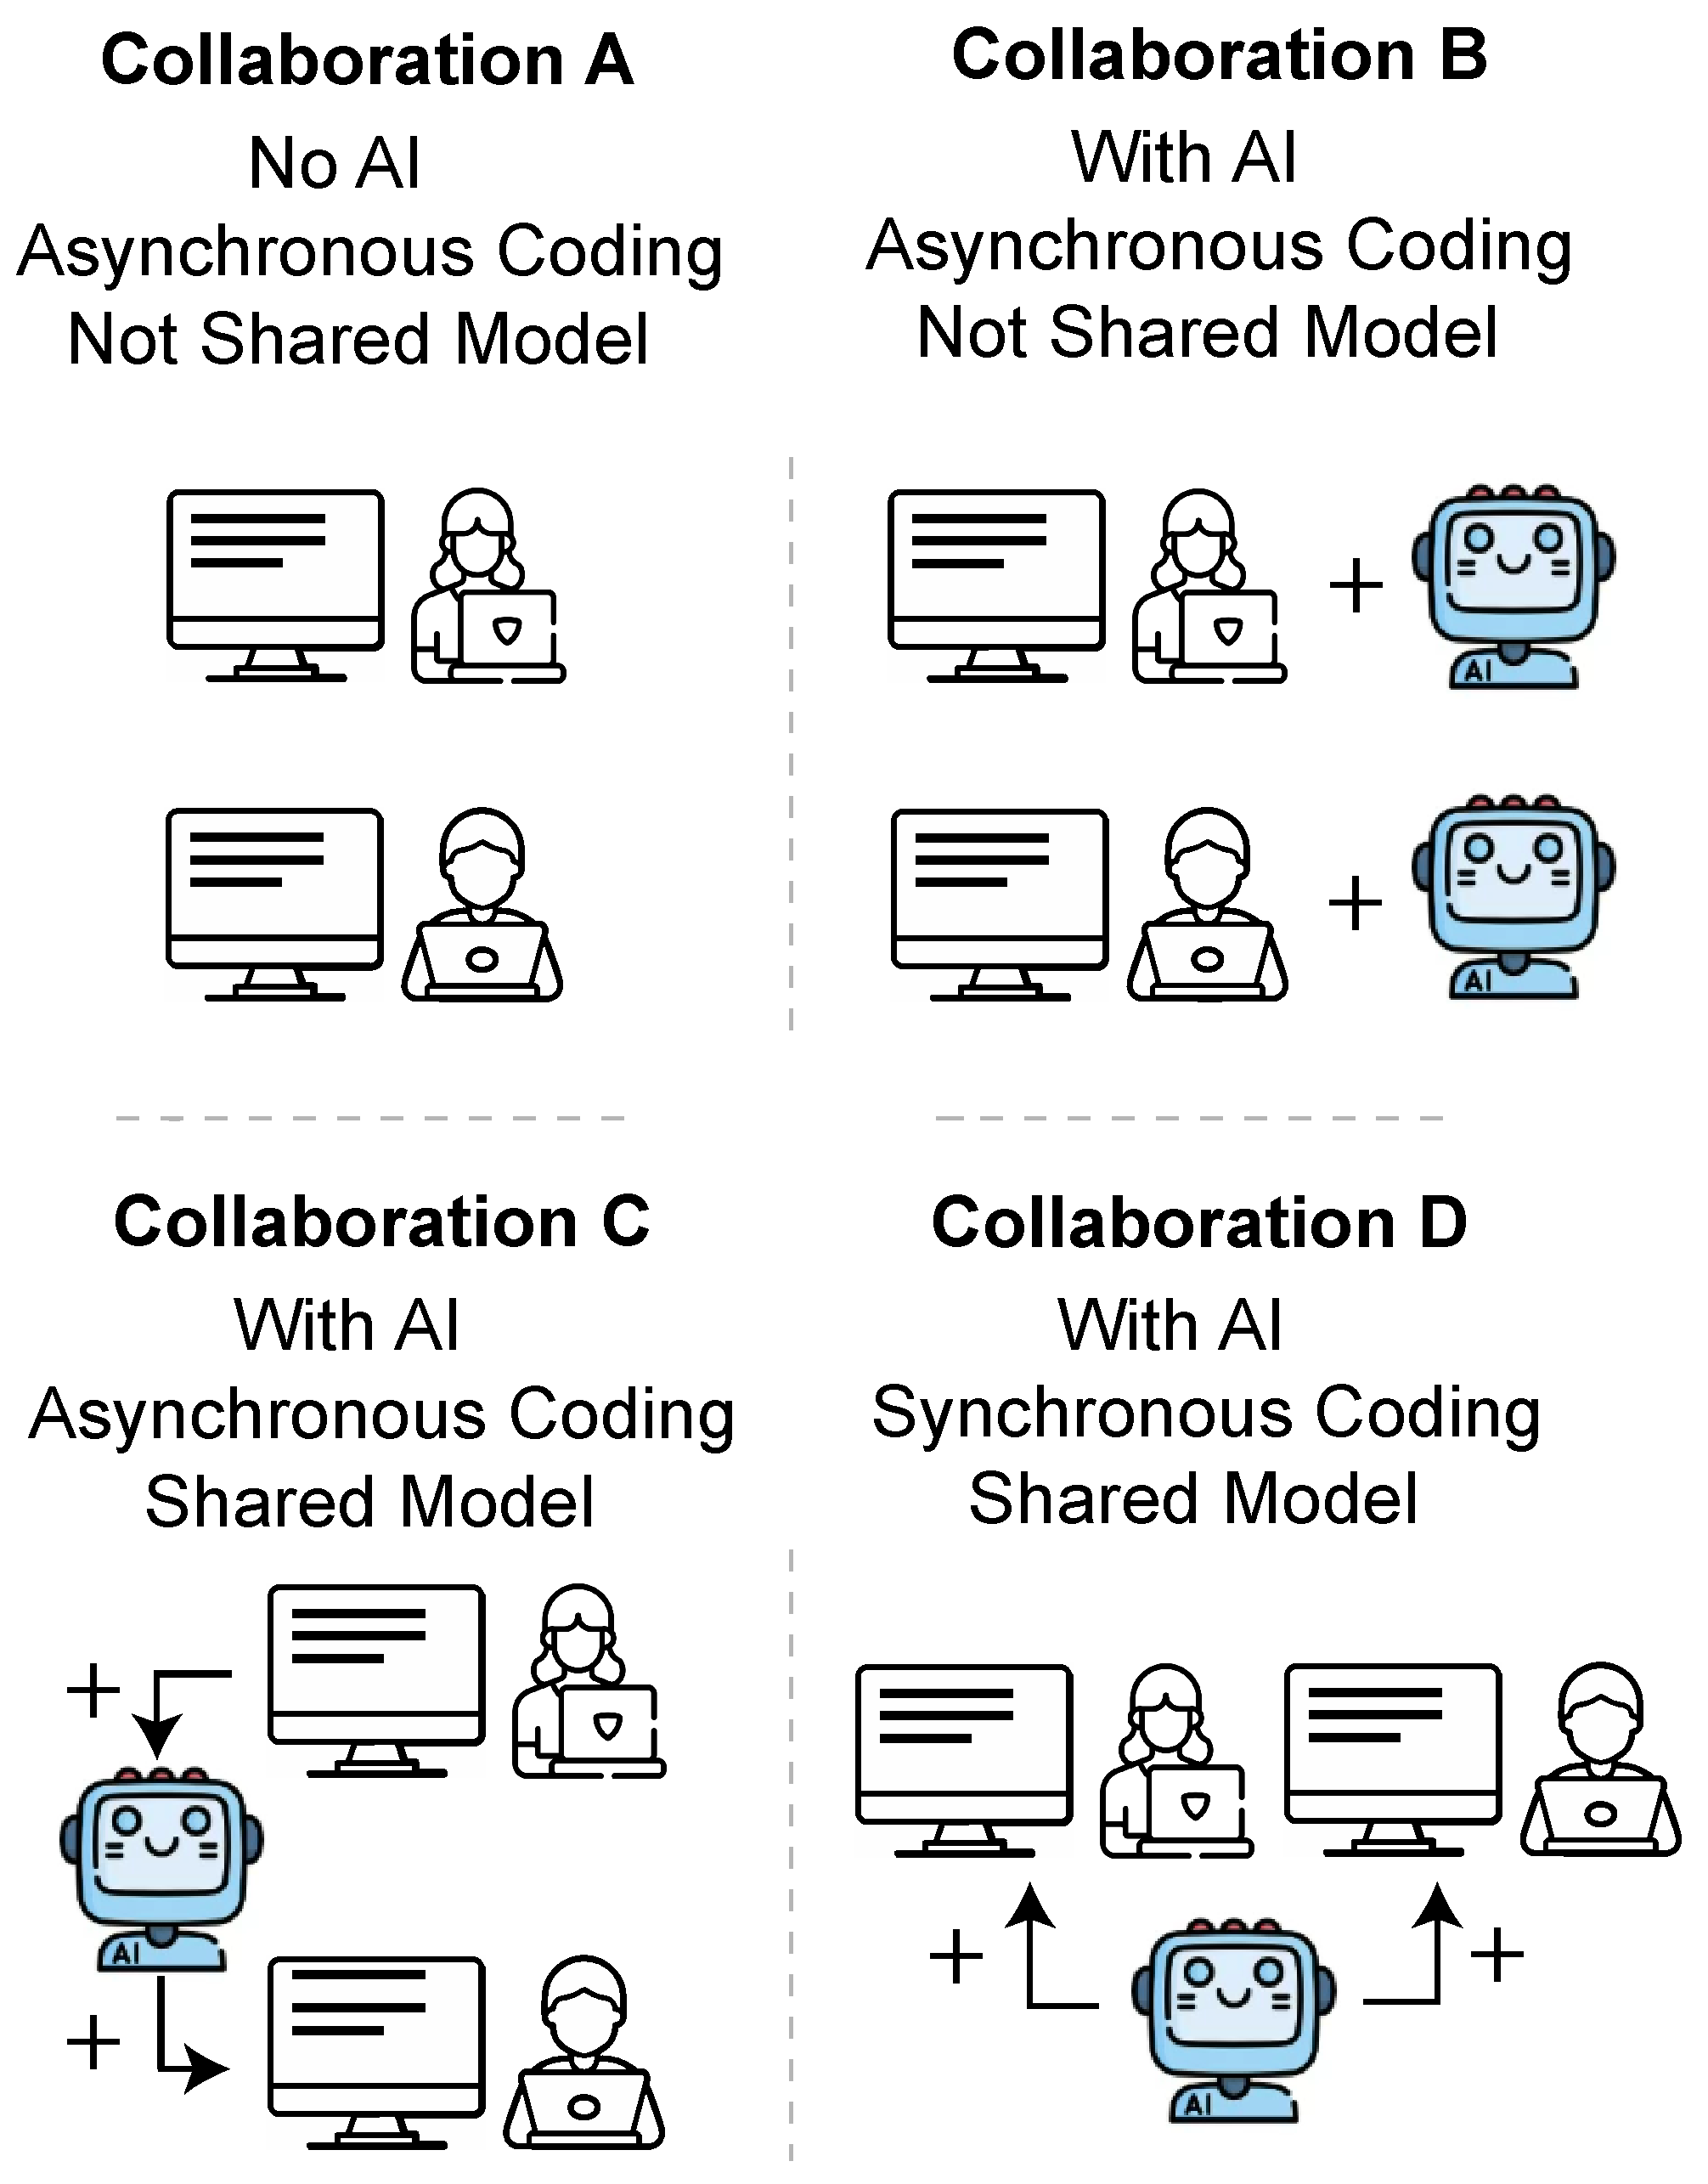
\includegraphics[width=0.4\textwidth]{collaboration_modes.pdf}
    \caption{Four collaborative modes of CQA~[1], three of which with AI integrated.}
    \label{fig:collab-modes}
    \vspace{-1em}
\end{wrapfigure}

\emph{First}, I aimed to develop a deep understanding of QDA practitioners' workflows, expectations, and practical challenges through in-depth interviews. Their feedback, particularly concerns about the inefficiency of collaborative practices, revealed that \emphtext{AI-assisted collaborative QDA was a critical yet underexplored area at the time}. What will happen if incorporating AI in the collaboration, what kind of integration is valid and feasible? \emph{Second}, I proposed designing \emphtext{AI systems not merely as tools, but as collaborative teammates}---capable of facilitating the resolution of interpretive discrepancies and fostering shared understanding among analysts. \emph{Third}, to evaluate the effectiveness of this approach, I conducted a human-subject study using a between-subjects design. This study examined four collaboration modes (Figure~\ref{fig:collab-modes}). Results show that while AI is promising for supporting efficient shared understanding, its impact depends on how it is integrated. A shared-model approach may suit efficiency-driven tasks, whereas individual models may better preserve analytical quality and agency. These findings offer design guidance for AI-supported collaboration contexts.

\newpage
\emphtext{Designing a solution for AI-powered QDA workflows~[2].} The integration strategy between AI and human analysts is critical, especially given the variability in QDA practices. To enable more reliable AI integration, I grounded the system design in established theoretical frameworks such as Grounded Theory and Thematic Analysis. I adopted a three-step approach. 

\begin{wrapfigure}{r}{0.32\textwidth}
    \vspace{-1em}
    \centering
    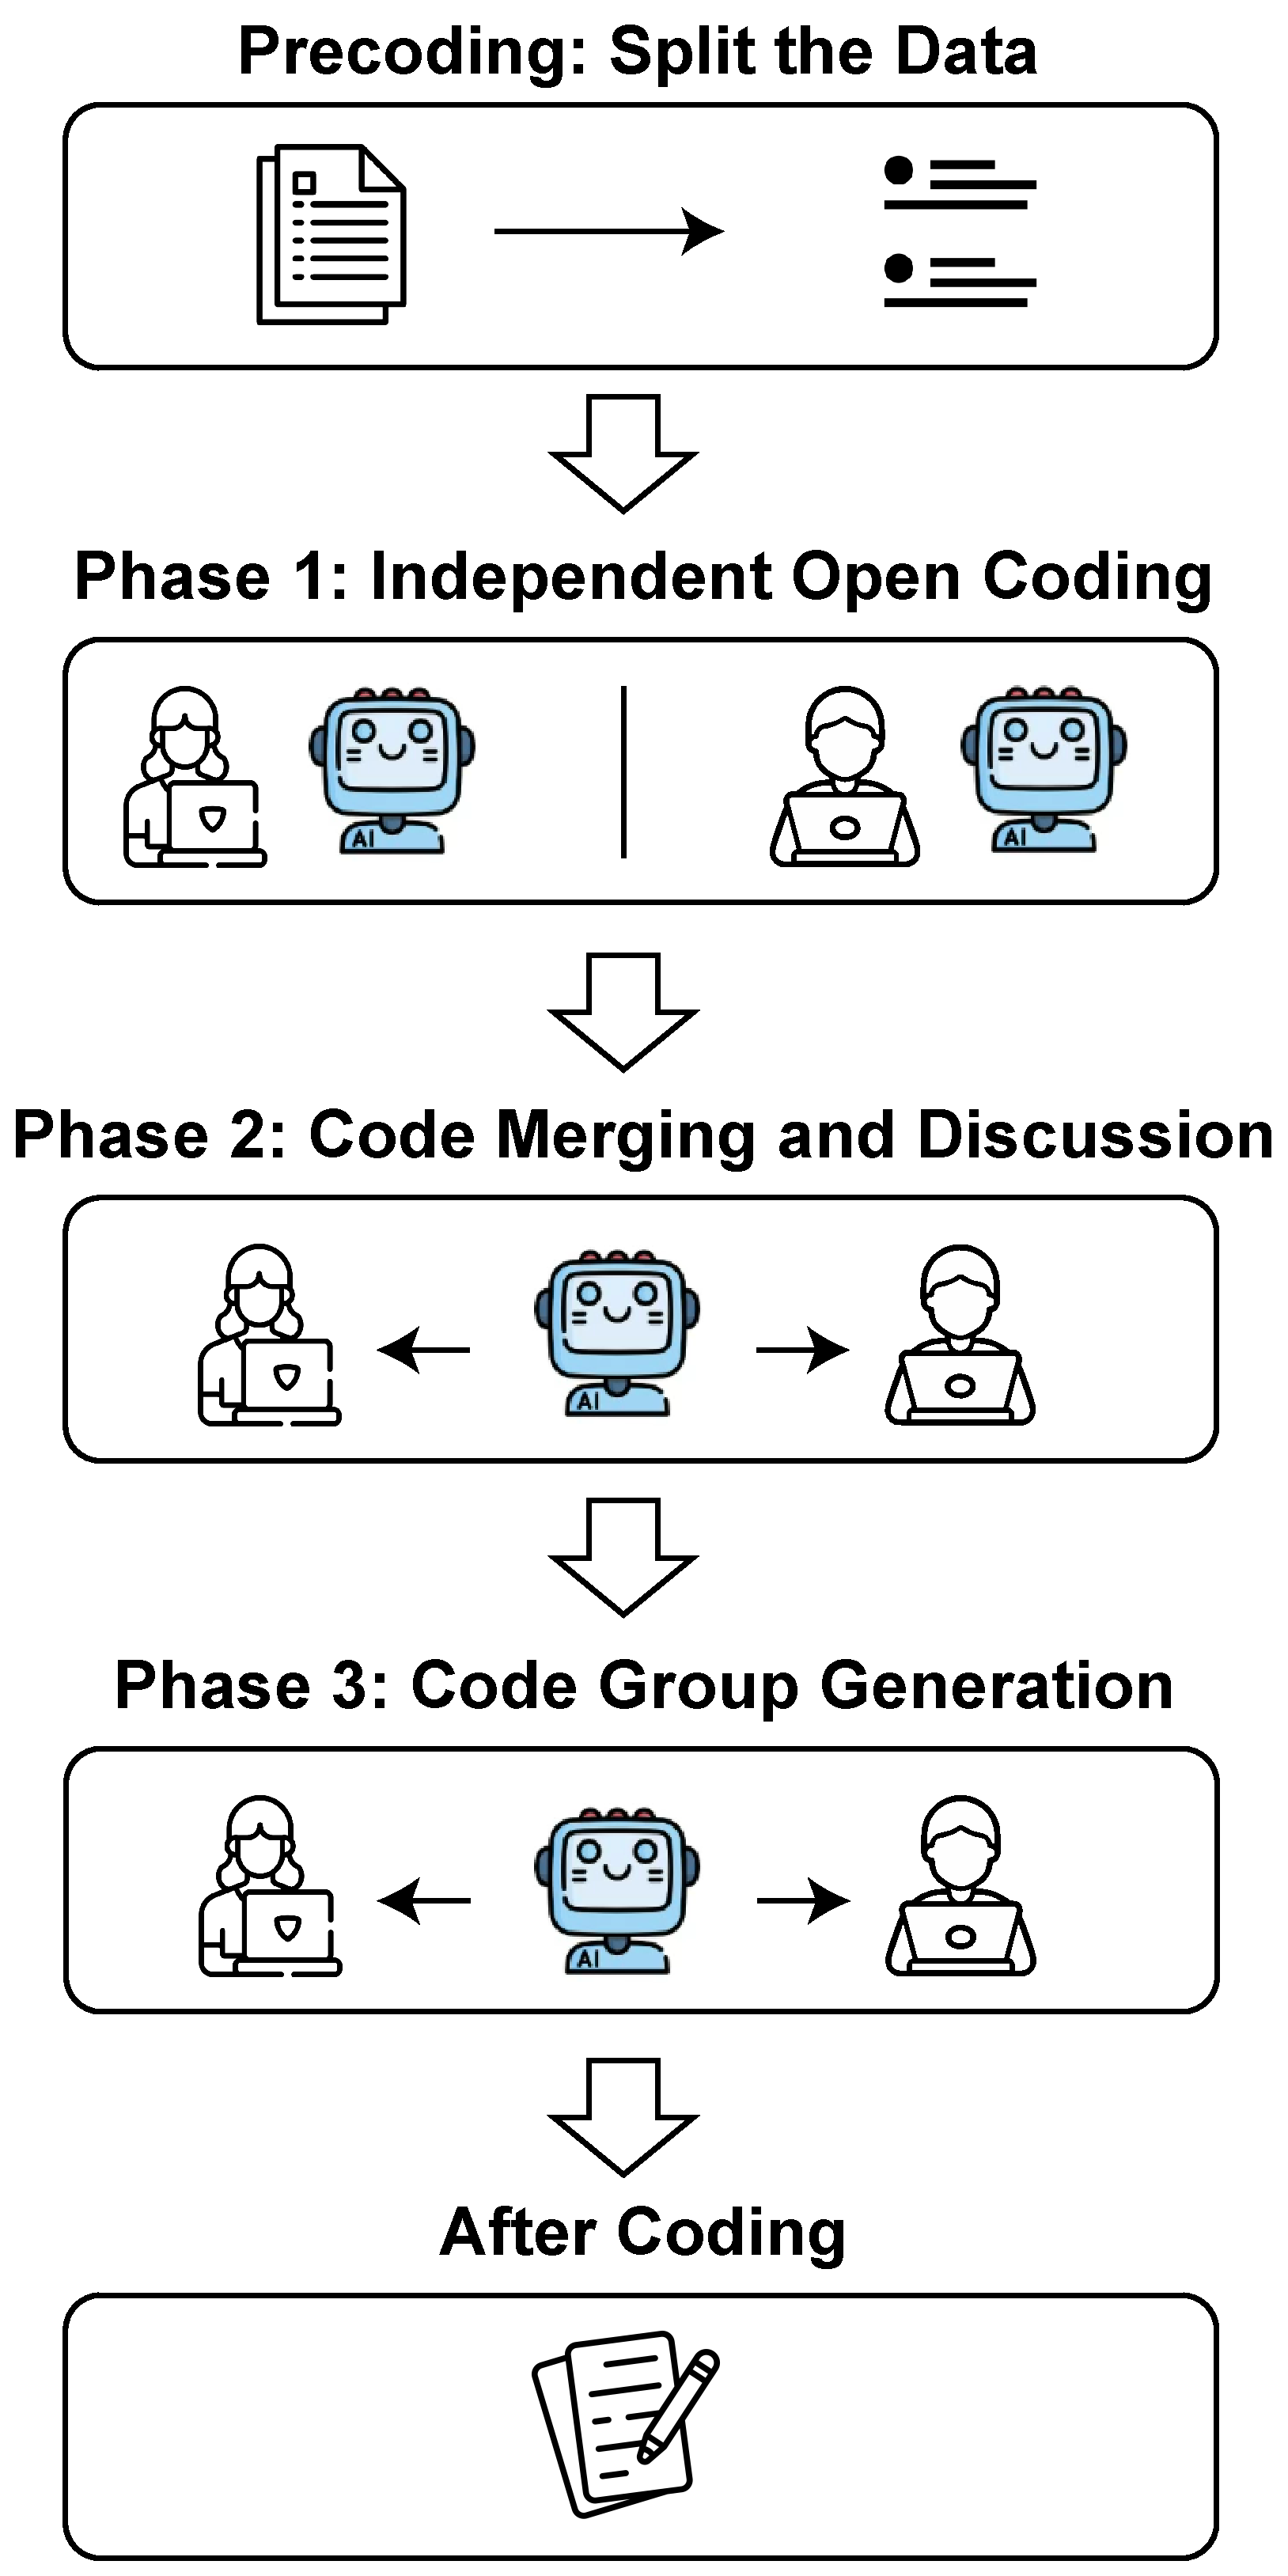
\includegraphics[width=0.3\textwidth]{collabcoder.pdf}
    \caption{A workflow~[2] that LLMs can support whole QDA pipeline.}
    \label{fig:collabcoder}
    \vspace{-1em}
\end{wrapfigure}

\emph{First}, through a semi-systematic literature review, user interviews, and analysis of existing QDA platforms, I identified eight design goals for AI-powered workflows. These include supporting varying levels of coding agency, iterative analysis, and transparent, collaborative workspaces. \emph{Second}, I translated these goals into a team-oriented workflow (Figure~\ref{fig:collabcoder}) that enables end-to-end collaboration with AI support at each stage, and developed the system as an open-source tool, \highlight{CollabCoder}. \emph{Third}, a within-subject user study showed that CollabCoder facilitates deeper discussions by surfacing coding disagreements and supporting the formulation of code groups, with \emphtext{LLMs acting as mediators and facilitators}. Furthermore, \emphtext{LLM as a suggestion provider} during individual coding helped reduce analysts' cognitive load in understanding text and framing qualitative code. However, those ``swift and less cautious'' pairs coded rapidly and appeared to rely overly on AI suggestions. These results showed that while integrating AI into human workflows offers clear benefits, such over-reliance may undermine the trustworthiness of results, particularly when AI generates substantial portions of the analysis. \emphtext{Ensuring trustworthy outcomes requires carefully balancing human agency and reliance on AI throughout the process.}

\subsection{Bring Humans to AI: Incorporating Humans into AI Generation}

\emphtext{Higher efficiency requires more automation, but at the cost of trustworthiness.} As AI models continue to advance in 2025, integrating them directly into human workflows like before can enhance efficiency while keeping humans in the loop. However, this approach is often constrained by human limitations and risks over-reliance when efficiency is prioritized. An emerging trend is to design prompt-based workflows where LLMs lead the entire coding process, offering significant gains in speed. Yet, such automation often yields unvalidated outputs and displaces human interpretation, resulting in outcomes that lack trustworthiness. \emphtext{How can we preserve essential human qualities, such as agency and interpretive judgment, within highly automated workflows?}

\begin{wrapfigure}{r}{0.35\textwidth}
    \vspace{-1em}
    \centering
    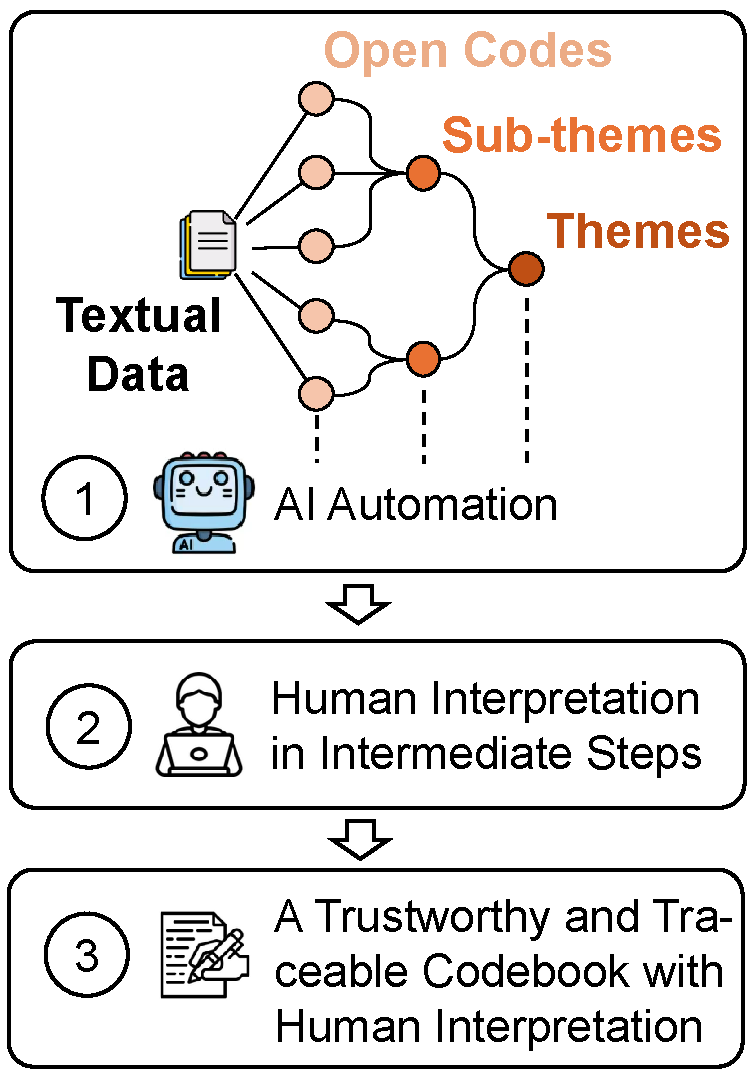
\includegraphics[width=0.33\textwidth]{mindcoder.pdf}
    \caption{AI automation optimized through appropriate human involvement.}
    \label{fig:mindcoder}
    \vspace{-1em}
\end{wrapfigure}

I proposed an approach to bring humans into AI driven automation through a core idea that \highlight{prioritizes verifiability over accuracy}~[3]. This approach was shaped through three steps from practitioner engagement to system implementation and evaluation. \emph{First}, to understand whether, how, when and where practitioners want to take part in the AI generation process, I conducted a semi-systematic literature review and practitioner interviews. These revealed several expectations for meaningful involvement, including preserving human agency, positioning humans as interpreters rather than validators, offering flexible engagement levels, encouraging active participation, and capturing analytical insights that can be reused. \emph{Second}, I implemented these principles in a publicly available web application, \highlight{MindCoder} (Figure~\ref{fig:mindcoder}), where AI automates basic-level grouping, humans critically reflect on intermediate outputs, and the system logs both AI- and human-generated results. Finally, the system produces a traceable, reusable, and human-verifiable PDF output that supports transparency and accountability throughout the process. \emph{Third}, a user study showed that the system enhanced user reflection, provided greater flexibility and control, and supported the production of results perceived as significantly more trustworthy.

% ============================================
% FUTURE RESEARCH AGENDA
% ============================================
\section{Future Research Agenda}

As a faculty member I plan to lead a research lab that advances the vision of \highlight{``placing humans at the center''} for AI-supported work so that human trust, agency, and user preferences remain central as automation grows. I will pursue this through three directions.

\subsection{System: Next-Generation Human--AI Collaborative Systems}

Recent AI-powered systems are expanding human-AI interaction across core cognitive activities such as reasoning and decision making. Tools like Cursor show how AI can generate intermediate plans that humans can inspect and refine, revealing a shift toward shared cognitive processes. Despite this progress, most systems still position AI as either a passive helper or a fully autonomous actor, and we lack a scientific account of how humans and AI should share cognitive responsibilities. This gap limits our ability to design reliable and interpretable collaboration at scale. My first research direction, grounded in my recent work~[5, 8], builds a theoretical and empirical foundation for the architecture of human-AI joint activity. I will study three questions. \emph{First}, what collaboration patterns reliably appear when humans and AI work together on complex tasks. \emph{Second}, how cognitive responsibilities can be allocated to preserve human autonomy and ownership while drawing on AI strengths. \emph{Third}, how to characterize capabilities that are uniquely human or uniquely AI and design workflows that allow both to excel. To advance these questions, I will integrate literature review, agent-based simulation, system building, and controlled studies. Literature review will surface stable collaboration patterns and cognitive bottlenecks. Agent simulations and system prototypes will make it possible to explore design tradeoffs and coordination strategies that are difficult to observe in human only settings. Controlled studies will validate the new tools. Together this direction will produce design principles and empirical evidence that guide the next generation of novel AI systems.

\subsection{Evaluation: Evaluation Frameworks for Human--AI Systems}

While existing research has explored how humans and AI can work together by designing new forms of collaboration, evaluating analytical outcomes remains an open challenge. Human judgments can be inconsistent, existing quality assurance frameworks are difficult to operationalize, and emerging approaches such as ``LLM-as-a-judge'' often lack grounding in human expectations. We still do not know which dimensions people should use to evaluate analytical outcomes, how to ensure quality at scale, or how to formalize interpretability and analytical rigor in ways that both humans and AI can apply. My third research direction, grounded in my ongoing work~[9], addresses this gap by developing frameworks for outcome quality evaluation. I will collaborate with experts in social science and psychology to construct theoretical frameworks rooted in qualitative research theory. I will build systems that instantiate these frameworks as scalable AI-based evaluators trained to approximate human criteria, and I will design hybrid human-AI evaluation workflows that preserve interpretive accountability while scaling to large datasets.

\subsection{Data: Broader Sensemaking Domains}

Many high value tasks in software engineering and AI research rely on cognitive processes similar to qualitative analysis. These include codebase understanding, analysis of AI agent trajectories, and more general multimodal information interpretation. Such tasks require people to read complex data, identify information of interest, and construct coherent understanding across distributed sources. Despite these shared cognitive processes, existing work rarely applies qualitative analysis methods or theories to these domains. This leaves several questions open. How can collaboration mechanisms developed for qualitative analysis be adapted to support sensemaking in code, agent behavior, or multimodal content. Which cognitive bottlenecks in these domains can be systematically supported by AI. How can AI transform raw complex information into representations that align with human reasoning strategies. My second research direction builds on my recent work on designing human AI collaboration for complex information extraction and presentation to developers~[4]. I will work closely with experts in software engineering and AI to study real workflows in these settings. I will combine interviews, controlled laboratory studies, quantitative analysis, and system building to examine how people understand complex information and how AI can support this process. The goal is to design collaborative scaffolds that generalize human AI collaboration beyond qualitative analysis and enable people to reason more effectively across diverse forms of complex data.

% ============================================
% REFERENCES
% ============================================
\newpage
\fancyfoot[C]{} % Remove page numbers from references
\section{References}

\begin{enumerate}[leftmargin=1.5em, itemsep=0.3em, label={[\arabic*]}]
    \item \textbf{Jie Gao}, Kenny Tsu Wei Choo, Junming Cao, Roy Ka-Wei Lee, and Simon Perrault. CoAICoder: Examining the effectiveness of AI-assisted human-to-human collaboration in qualitative analysis. \emph{ACM Transaction on Computer Human Interaction (TOCHI)}, 2023. \url{https://doi.org/10.1145/3617362}.
    
    \item \textbf{Jie Gao}, Yuchen Guo, Gionnieve Lim, Tianqin Zhang, Zheng Zhang, Toby Jia-Jun Li, and Simon Tangi Perrault. CollabCoder: A lower-barrier, rigorous workflow for inductive collaborative qualitative analysis with large language models. In \emph{Proceedings of the 2024 CHI Conference on Human Factors in Computing Systems (CHI24)}, 2024. \url{https://doi.org/10.1145/3613904.3642002}.

    
    \item \textbf{Jie Gao}, Yue Xue, Xiaofei Xie, SoeMin Thant, Erika Lee, and Bowen Xu. Understanding codebase like a professional! Human-AI collaboration for code comprehension, 2026. \url{https://arxiv.org/abs/2504.04553}. Accepted at the 34th IEEE/ACM International Conference on Program Comprehension (ICPC 2026).

    \item \textbf{Jie Gao}, Simret Araya Gebreegziabher, Kenny Tsu Wei Choo, Toby Jia-Jun Li, Simon Tangi Perrault, and Thomas W Malone. A taxonomy for human-LLM interaction modes: An initial exploration. In \emph{Extended Abstracts of the CHI Conference on Human Factors in Computing Systems}, CHI EA '24. \url{https://doi.org/10.1145/3613905.3650786}.

    \item \textbf{Jie Gao}, Xiayin Ying, Junming Cao, Yifan Yang, Pin Sym Foong, and Simon Perrault. Differences of challenges of working from home (WFH) between Weibo and Twitter users during COVID-19. In \emph{Extended Abstracts of the 2022 CHI Conference on Human Factors in Computing Systems}, CHI EA '22, 2022. \url{https://doi.org/10.1145/3491101.3519790}.

    \item \textbf{Jie Gao}, Zhiyao Shu, Shun Yi Yeo, Alok Prakash, Chien-Ming Huang, Mark Dredze, and Ziang Xiao. Efficiency with rigor! A trustworthy LLM-powered workflow for qualitative data analysis, 2025. \url{https://arxiv.org/abs/2501.00775}. \noindent\colorbox{accentcolor}{\textbf{\textcolor{white}{In submission.}}}

     \item \textbf{Jie Gao}, Thomas Malone, et al. Not just prompt engineering: A taxonomy for human LLM interaction modes, 2025. \noindent\colorbox{accentcolor}{\textbf{\textcolor{white}{In preparation.}}}
    
    \item \textbf{Jie Gao}, Mian Zhong, Jonathan Ivey, Chien Ming Huang, Ziang Xiao, and Mark Dredze. Evaluation framework for LLM assisted qualitative data analysis, 2025. \noindent\colorbox{accentcolor}{\textbf{\textcolor{white}{In preparation.}}}

     \item Zheng Zhang, \textbf{Jie Gao}, Ranjodh Singh Dhaliwal, and Toby Jia-Jun Li. VISAR: A human-AI argumentative writing assistant with visual programming and rapid draft prototyping. In \emph{Proceedings of the 36th Annual ACM Symposium on User Interface Software and Technology}, UIST '23, 2023. \url{https://doi.org/10.1145/3586183.3606800}.

      \item ShunYi Yeo, Gionnieve Lim, \textbf{Jie Gao}, Weiyu Zhang, and Simon Tangi Perrault. Help me reflect: Leveraging self-reflection interface nudges to enhance deliberativeness on online deliberation platforms. In \emph{Proceedings of the 2024 CHI Conference on Human Factors in Computing Systems}, CHI '24, 2024. \url{https://doi.org/10.1145/3613904.3642530}.
    
    \item Marianne Aubin Le Quéré, Hope Schroeder, Casey Randazzo, \textbf{Jie Gao}, Ziv Epstein, Simon Tangi Perrault, David Mimno, Louise Barkhuus, and Hanlin Li. LLMs as research tools: Applications and evaluations in HCI data work. In \emph{Extended Abstracts of the CHI Conference on Human Factors in Computing Systems}, CHI EA '24. \url{https://doi.org/10.1145/3613905.3636301}.

    
   
    
    \item Junming Cao, Bihuan Chen, Longjie Hu, \textbf{Jie Gao}, Kaifeng Huang, Xuezhi Song, and Xin Peng. Characterizing the complexity and its impact on testing in ML-enabled systems. In \emph{2023 IEEE International Conference on Software Maintenance and Evolution (ICSME)}. \url{https://doi.org/10.1109/ICSME58846.2023.00034}.
    
   
    
    \item Ruyuan Wan, Haonan Wang, Ting-Hao Kenneth Huang, and \textbf{Jie Gao}. From noise to nuance: Enriching subjective data annotation through qualitative analysis. In \emph{Proceedings of the Fourth Workshop on Bridging Human-Computer Interaction and Natural Language Processing (HCI+NLP)}, 2025. \url{https://aclanthology.org/2025.hcinlp-1.20/}.
\end{enumerate}

\end{document}
